Den Zeeman-Effekt unterscheidet man durch seine \emph{normale} und \emph{anomale} Version, wobei erstere effektiv unter Spinvernachlässigung und letztere unter Spinberücksichtigung Aussagen über die Spektralaufspaltung trifft. Aus Sicht der klassischen Elektronenanschauung zerlegt man ein um den Atomkern oszillierendes Atom in drei Anschauungselektronen mit (i) linearer, (ii) positiver und (iii) negativer zirkularer Oszillation. Hierbei wird die Aufteilung unter Berücksichtigung des anliegenden linearen $B_0$ Feldes vorgenommen, wie Abbildung \ref{fig:ElektronOszillationZerlegung} zeigt. 
\begin{figure}[H]
	\centering
	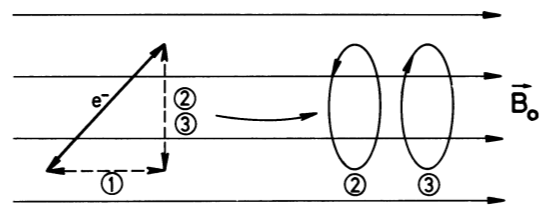
\includegraphics[width=5cm]{../../Bilddateien/Grundlagen/ElektronOszillationZerlegung.png}
	\label{fig:ElektronenOszillationZerlegung}
	\caption{Zerlegung der Elektronenoszillation in drei Anschauungselektronen.}
\end{figure}
Im Fall (i) finden wir $E\parallel B_0$ und keinerlei Frequenzänderung. Die Fälle (ii) und (iii) erfahren durch eine Änderung des Magnetfeldes jedoch mittels Induktion eine Beschleunigung, dessen Vorzeichen von der Umlaufrichtung abhängig ist. Der Betrag der Frequenzänderung ist dabei für $\mu_B$ als \emph{Bohrsches Magneton} gegeben durch 
\[
	\Delta\omega = \frac{\mu_B}{\hbar}\cdot\dabs{B_0}{}.
\]
Dies zeigt man im Wesentlichen durch Gleichsetzung der Coulomb- und Zentrifugalkräfte des Elektrons und kartesischer Zerlegung der so entstehenden Bewegungsgleichungen. Das entscheidende Ergebnis dieser Berechnungen ist jedoch der \emph{konstante} Aufspaltungsabstan einer Spektrallinie in drei äquidistante Linien, was durch dieses Modell beschrieben ist. Die Emissionsrichtung ist dabei durch die Magnetfeldrichtung gegeben. 
